\chapter{Review of Fundamentals}

\section{Sinusoids}

A sinusoid is a time function of the form
\[
  A \sin(\omega t + \phi)
\]
where

\begin{tabular}{ccc}
$A$   &  Amplitude  &  Volts, Amps, etc \\
$\omega$   & Frequency  & $rad/sec$ \\
$t$     & Time  & $sec$  \\
$\phi$  & Phase & $rad$  \\
\end{tabular}

Sinusoids arise in ECE through two primary ways

1) The mathematical solutions to circuits built-up of R, L, C elements sometimes
contain sinusoidal terms.

2) Rotating machines like generators can generate sinusoidal voltages.

Some properties of sinusoids include:

Since $\omega$ is in $rad/sec$, we must frequently convert frequencies in cycles per second (Hertz)
by noting that one cycle is $2\pi$ radians thus for edxample:

  \[
    1000 Hz = 2\pi\times 1000 \approx 6283.2 rad/sec
    \]

The Phase angle, $\phi$, slides the sinusoid back and forth along the time axis acording to its value
(which is a constant).  There are special cases when $\phi$ is a multiple of $\pi/2$ such as
\[
  A \sin(\omega t + \pi/2) = -A \cos(\omega t)
  \]

or
\[
  A \sin(\omega t + \pi) = -A \sin(\omega t)
  \]
according to various trig identities.

Since $\sin()$ and $\cos()$ have important geometrical interpretations, it is not surprinsing that it is often useful to
visualize a sinusoid as a projection of a rotating vector onto the $X$ or $Y$ axis.

***********    Illustration



\subsection*{Sinusoid Review}

%\includegraphics[width=0.5\textwidth]{sinusoid_graph.png}

\begin{enumerate}
\item Find time where $\theta = 0$ (because $\cos(0) = 1$)

at $t = 0$, $t = 0$

\item Find line where $\theta = \pi/2$ (because $\cos(\pi/2) = 0$)

at $t = \pi/2$, $t = \pi/6$

\item "$\theta = \pi$ (" $\cos(\pi) = -1$)

at $t = \pi$, $t = \pi/3$

etc.

So goal: $\cos(\omega t + \phi)$

A

$(1) \omega t + \phi = 0$
$t = -\phi/\omega$

$(2) \omega t + \phi = \pi/2$
$\omega t = \pi/2 - \phi$
$t = \frac{\pi/2 - \phi}{\omega}$

etc
\end{enumerate}


\section{Complex Numbers}


Complex numbers make use of the famous imaginary number
$i = \sqrt{-1}$.    In ECE that is confusing with current so we use instead
\[
  j = \sqrt{-1}
\]

An {\it imaginary} number is any real number multiplied by $j$ such as
\[
10j,\; -4j,\; 14.7j, \; \mathrm{etc.}
\]

A {\it complex} number is the sum of a real number plus an imaginary number:
\[
  Z = a + bj
\]

\subsection{Complex Plane}

We represent complex numbers in the {\it Complex Plane}.   The complex plane is
a version of the $X,Y$ plane where each complex number represents a point or vector in
which its real part is the $X$ coordinate and its imaginary part is the $Y$ coordinate.

For example the two complex numbers

\[
Z_1 = 2 + 3j, \quad Z_2=-1-3j
\]
can be drawn on the complex plane below as:

[Graphic]
%\includegraphics[width=0.5\textwidth]{MR6732.png}

Like any plane, the complex plane can also be addressed in polar coordinate form.

\begin{align}
Z &= a + bj & &= r\angle\theta \\
a &= \text{Re}\{Z\} & r &= \sqrt{a^2+b^2} & \text{Magnitude} \\
b &= \text{Im}\{Z\} & \theta &= \tan^{-1}\left(\frac{b}{a}\right) & \text{Angle}
\end{align}


\subsection{Exponential Form}

One of the most famous equations in mathematics is Euler's Identity:
\begin{equation}
\boxed{e^{j\theta} = \cos(\theta) + j\sin(\theta)}
\end{equation}

\begin{equation}
e^{j\pi} = -1
\end{equation}



\subsection{ Computation with Complex Numbers}

\noindent Rectangular Form:
\begin{align}
\text{Addition:} \quad       & $(a + bj) + (c + dj) = (a+c) + (b+d)j$ \\
\text{Multiplication:} \quad &(a + bj) \times (c + dj) = ac + adj + bcj + bdj^2 = ac-bd + (ad+bc)j$
\end{align}

\noindent Polar Form:
\begin{align}
\text{Addition:} \quad  &$r_1\angle\theta_1 + r_2\angle\theta_2$ \text{add like vectors} \\
\text{Multiplication:} \quad & (r_1\angle\theta_1)\times(r_2\angle{\theta_2 = r_1r_2\angle(\theta_1+\theta_2)
\end{align}

So each operation (addition or Multiplication) is easiest in one of the two forms, summed up with the slogan
\begin{quotation}``Angles add, Magnitudes multiply''\end{quotation}

\noindent{Exponential Form}
Note that the polar form is derived from Euler's exponential form:
\begin{align}
\text{Addition:} \quad &\text{Euler's $e^{j\alpha}$} \\
\text{Multiply:} \quad &A_1e^{j\theta_1} \cdot A_2e^{j\theta_2} = A_1A_2e^{j(\theta_1+\theta_2)}
\end{align}



\subsection{Complex Conjugate}
If $Z = a + jb$ then its complex conjugate, $Z^* = a - jb $, in other words to get the Complex conjugate of  a complex
number, just multiply its imaginary part by $-1$.
If we multiply a complex number by its conjugate, it is easy to see that we get its Magnitude:

\[
ZZ^* =  (a+bj)(a-bj) = a^2 - abj + abj - b^2j^2 = a^2 + b^2
\]

[Graphic]
%\includegraphics[width=0.5\textwidth]{MR6733.png}


\begin{align}
\text{e.g. Division:} \quad \frac{Z_1}{Z_2} &= \frac{a_1 + b_1j}{a_2 + b_2j} = \frac{Z_1 \cdot Z_2^*}{Z_2 \cdot Z_2^*} = \frac{Z_1Z_2^*}{|Z_2|^2}
\end{align}

\subsection*{Complex Number Arithmetic in a nutshell:}
\begin{tabular}{l|p{1.in}|p{1.0in}|p{1.0in}}
Form                 & Add           & Multiply           & Conjugate \\\hline
Rectangular, $a+bj$  & By Component  & Like a Polynomial  & Negate imaginary part\\ \hline
Polar,
$A\angle{\theta}$    & like Vectors  & Angles Add, Magnitudes Multiply & Negate Angle \\ \hline
Exponential,
$Ae^{j\theta}$       & Convert to rectangular! & just like Polar & Negate exponent
\end{tabular}

\subsection{Examples}

Q: What is $\sqrt{-64}$?

A: $\sqrt{-1 \cdot 64} = \sqrt{-1} \cdot 8 = j8$ or imaginary \#

Q: What is $2 + j\sqrt{-36}$?

A: $2 + j6$, can't be simplified; solution is
a Complex \# that can be considered to
be a projection of a (rotating) vector.

\noindent at $t=0$

%\includegraphics[width=0.5\textwidth]{vector_diagram.png}

Therefore, their sum is the projection of their vector
sum:

\noindent{\bf Caution: start}
$r = \sqrt{8^2 + 6^2} = \sqrt{64 + 48} = 10.6$

$\theta = \tan^{-1}\left(\frac{6}{8}\right) = 41^\circ = .71 \text{ rad}$
\noindent{\bf Caution: end}

$8\cos(\omega t + 7/2) + 6\cos(\omega t) = 10.6\cos(\omega t + 0.71)$


\clearpage
\newpage
%%%%%%%%%%%%%%%%%%%%%%%%%%%%%%%%%%%%%%%%%%%%%%%%%%%%%%%%%%%%%%%%%%%%%%%%%%%%%%%%%%%%%%%%%%%%%%%%%%%%%%%%%%%%%%%%%%%%%%
\section{Complex Number Quiz}\label{ComplexNumberQuiz}
Take this quiz then check your answers on Page \pageref{CN_answers}.  Use only the following functions on your calculator (or fewer as instructed):

\[
* \quad \div + \quad - \quad \sqrt{x}
\]


It should be {\bf easy for you to get exact answers}.  If not, then you need to review the concepts in this quiz and section \ref{cnconcepts}.   Some Kahn Academy videos are pre-linked in Section \ref{KahnV}.


\begin{enumerate}

\item  What is $\sqrt{-16}$ ?

\item  Evaluate
\[
X = \frac{-b + \sqrt{4ac}}{2a}
\]
for the following values:
\begin{quotation}
\begin{tabular} {c|c|c}
a&b&c  \\ \hline
1&2&3 \\
1&-4&29\\
2&28&1156
\end{tabular}
\end{quotation}


\item  Evaluate
\[
(6+j16) + (-7-j6) =
\]
\[
(27-j0.75) - (1.6+j0.27) =
\]


\item  Evaluate  $M\times N$ where

\begin{quotation}
\begin{tabular} {c|c}
M&N \\ \hline
$(2+6j)$	&	$(1+3j)$   	\\
$(1.7-0.6j)$    &	$(3.2+0.4j)$	\\
\end{tabular}
\end{quotation}


\item  Plot the following points on the complex plane:
\[
a = -3+1.5j \qquad b = 2-j \qquad c = j
\]


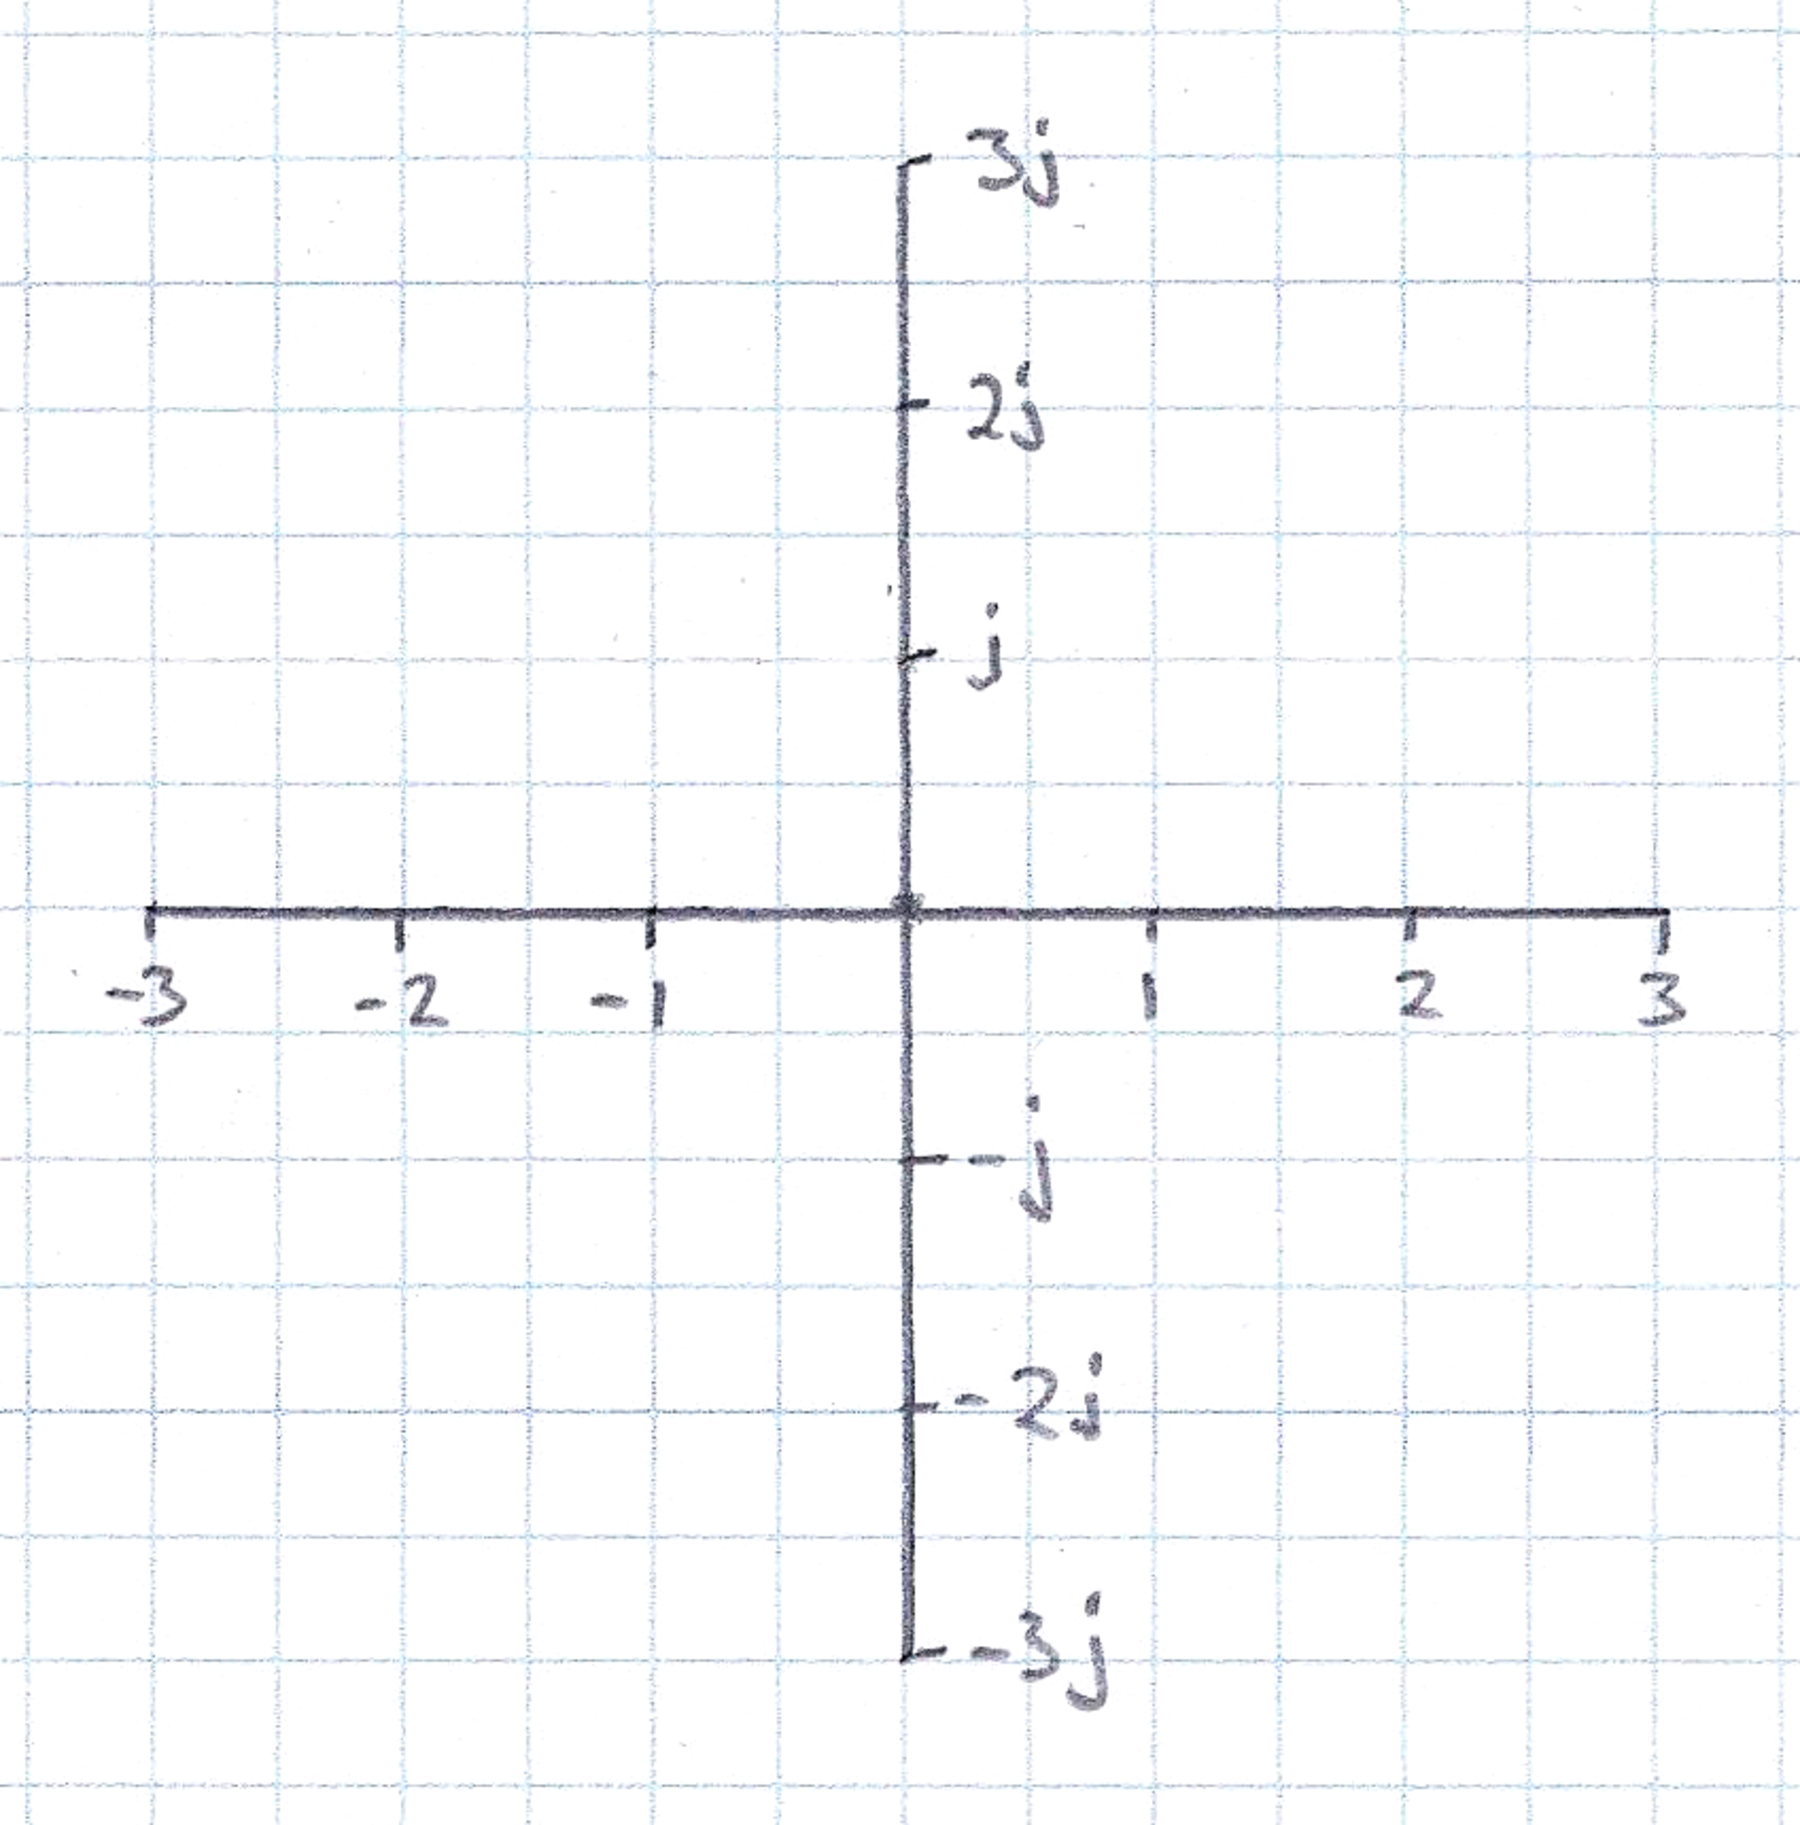
\includegraphics[width=6cm]{figsapdx/00926a.png}



\item  Convert $X_1=(4+3j)$ to polar (magnitude-angle) form


\item  Convert $X_2=(-16+3.7j)$ to polar (magnitude-angle) form


\item  Represent $X_3 = (-1+6j)$ in exponential form

\item  For
\[
a = 3e^{j\pi/4} \qquad b = 2\angle{45^\circ}
\]
Convert them to ``$a+bj$'' form and multiply $a*b$ without using a calculator.

\end{enumerate}








\section{Complex Number Concepts required for EE233}\label{cnconcepts}
\begin{itemize}
  \item $j = \sqrt{-1}$
  \item complex number is the sum of a real part, $\sigma$ + an imaginary part $j\omega$ (where $\omega$ is a real number to be multiplied by $j$.)
  \item   The {\it magnitude} of a complex number is the Pythagorean sum of the real and imaginary parts:
  If $x= a+jb$ is a complex number, then the magnitude is
  \[
  |x| = \sqrt{a^2+b^2}
  \]
  \item To add together two complex numbers, add their real and imaginary parts separately.
  \[
  x = a+bj \qquad y = c+dj
  \]
  \[
  x + y = (a+c) + j(b+d)
  \]
  \item To multiply two complex numbers, multiply them together like two first order polynomials in $j$ (using the definitions above)
  \[
  x*y = (a+bj)*(c+dj) = ac+adj + bcj+bdj^2
  \]
  since $j^2=-1$ we have
  \[
  x*y = (ac-bd)+(ad+bc)j
  \]

  \item Complex numbers describe a point in the {\it complex plane}.  The $X$ axis of the complex plain is the real part of the complex number and the $Y$ axis is the imaginary part.

  \item To plot the point $a+jb$ on the complex plane, plot a point at $X = a, \: Y = b$.

  \item The magnitude of a complex number is the distance from the origin to its point on the complex plane.

  \item The {\it angle} of a complex number is the angle formed from the positive real axis ($X>0$) and the line between the origin and the point.

  \item There is an \href{http://en.wikipedia.org/wiki/Euler\%27s_formula}{exponential form} of any complex number:
  \[
  e^{j\theta} = \cos(\theta) + j\sin(\theta)
  \]
  \item To convert a complex number to exponential form we invert the previous equation:
  \[
  a+bj = |a+bj| e^{j\tan^{-1}(b/a)}
  \]

  \item The $\tan^{-1}()$ function traditionally limits us to quadrants I and IV of the complex plain.    More generally we can use the 4-quadrant 2-argument arctan function \href{http://en.wikipedia.org/wiki/Atan2}{({\tt atan2(b,a)}) }.

  \item A consequence of multiplication of complex numbers and the exponential represenation of complex numbers is that when we multiply two complex numbers:
     \begin{quotation} {\it ``angles add and magnitudes multiply''}
     \end{quotation}
   if $A,B,C$ are complex numbers and $C = A * B$
   \[
    \angle{C} = \angle{A}+\angle{B}  \qquad   |C| = |A|*|B|
   \]


\end{itemize}

\section{Kahn Academy Videos}\label{KahnV}

\href{https://www.khanacademy.org/math/algebra/complex-numbers/complex_numbers/v/complex-numbers}{complex numbers}

\href{https://www.khanacademy.org/math/trigonometry/imaginary_complex_precalc/complex_analysis/v/exponential-form-to-find-complex-roots}{exponential form of complex numbers}








\section{Kirchoff's Current and Voltage Laws (KCL, KVL)}

\subsection{KCL}
In our context we can express KCL as follows:

If a node connects $n$ conductors having currents, $i_1 \dots i_n$,
then
\[
\sum_k i_k = 0
\]
Physically this means that charge cannot accumulate on a node and give it a
potential (of course a capacitor {\it can} accumulate charge!).

\subsection{KVL}
Our version of KVL states:

If a circuit loop, consists of $n$ nodes (which may belong to other loops as well),
and we define the $k^{th}$ branch as the branch connecting node $k$ with node $k-1$, and if $V_k$ is defined as the voltage drop across the branch:
\[
V_k = v_k - v_{k-1}
\]
(where $v_k$ is the voltage at node $k$)
then KVL is
\[
\sum_k V_k = 0
\]
In words, the sum of the voltage drops around any loop is equal to zero. In an
every day example, if you walk any closed path around the streets of Seattle,
your net gain in elevation (net change of potential energy) must be zero.

For more complex circuits having more than one node or loop,
KCL and KVL are frequently used to generate a set of equations which can be
jointly solved to get all the node voltages or branch currents.



\section{Basic Operational Amplifier Configurations}


\subsection{Inverting Amplifier}
\subsection{Non-inverting Amplifier}
\subsection{Summing Amplifier}
\subsection{Voltage Follower}

\section{deciBells (dB)}

\section{2, and 4 quadrant arc-tangent functions}

\section{Voltage Dividers}

\section{Thevenin and Norton equivalent circuits}

